%\documentclass[5p, sort&compress]{elsarticle}
\documentclass[sort&compress]{elsarticle}
%\documentclass{cas-sc}
\usepackage[utf8]{inputenc}
\usepackage{amsmath}
\usepackage{amssymb}{}
\usepackage{amsthm}
\usepackage{enumerate}
\usepackage{lineno, hyperref}
\usepackage{listings}
\usepackage{booktabs}
\usepackage{siunitx}
\usepackage{graphicx}
\usepackage[nameinlink,noabbrev]{cleveref}
\usepackage[draft]{changes}
\usepackage[section]{placeins}

\usepackage[]{algorithm,algcompatible,lipsum}
\usepackage[]{algpseudocode}

\modulolinenumbers[1]
\definechangesauthor[color=orange]{SDIV}
\linenumbers
\newdefinition{hypotheses}{Hypothesis}
\newdefinition{assumptions}{Assumptions}
\begin{document}
    %%!TEX root = main.tex
\begin{frontmatter}
    \title{
        Picewise Constant Optimal Vaccination policies for COVID-19
    }
    %%%%%%%%%%%%%%%%\textbf{}%%%%%%%%%%%%%%%%%%%%%%%%%%%%%%%%%%%%%%%%%%%%
    \author[add:unison]%
    {Gabriel A. Salcedo-Varela}
    \ead{avarela155@gmail.com}
    \address[add:unison]{
        Departamento de Matem\'aticas, Universidad de Sonora,
        Blvd. Luis Encinas y Rosales S/N,
        Hermosillo, Sonora, M\'exico, C.P. 83000.
    }
    %%%%%%%%%%%%%%%%%%%%%%%%%%%%%%%%%%%%%%%%%%%%%%%%%%%%%%%%%%%%%%%%
    \author[add:UADY]%
    {Francisco Pe\~nu\~nuri}
    \ead{francisco.pa@uady.mx}
    \address[add:UADY]{Facultad de Ingenier\'ia, Universidad 
    Aut\'onoma de Yucat\'an, A.P. 150, Cordemex, M\'erida, Yucat\'an, 
    M\'exico.}
    %%%%%%%%%%%%%%%%%%%%%%%%%%%%%%%%%%%%%%%%%%%%%%%%%%%%%%%%%%%%%%%%
    \author[add:conacyt_unison]{D. Gonz\'alez-S\'anchez}
    \ead{dgonzalezsa@conacyt.mx}
        \address[add:conacyt_unison]{
        CONACYT-Universidad de Sonora,
        Departamento de Matem\'aticas,
        Blvd. Luis Encinas y Rosales S/N,
        Hermosillo, Sonora, M\'exico, C.P. 83000.
    }
    %%%%%%%%%%%%%%%%%%%%%%%%%%%%%%%%%%%%%%%%%%%%%%%%%%%%%%%%%%%%%%%%
    \author[add:conacyt_unison]{%
        Sa\'ul D\'iaz-Infante%
        \corref{corresponding_author}%
    }%
    \ead{saul.diazinfante@unison.mx}
    %%%%%%%%%%%%%%%%%%%%%%%%%%%%%%%%%%%%%%%%%%%%%%%%%%%%%%%%%%%%%%%
    \cortext[corresponding_author]{Corresponding author}
    \journal{Annual Reviews in Control}
    %!TEX root = main.tex
\begin{abstract}
We formulate a controlled system of ordinary differential equations, with
vaccination and lockdown interventions as controls, to simulate the mitigation
of COVID-19. The performance of the controls is measured through a cost
functional involving vaccination and lockdown costs as well as the burden of
COVID19 quantified in DALYs. We calibrate parameters with data from Mexico City
and Valle de Mexico.  By using differential evolution, we minimize the cost
functional subject to the controlled system and find optimal policies that are
constant in time intervals of a given size. The main advantage of these
policies relies on its practical implementation since the health authority has
to make only a finite number of different decisions. Our methodology to find
optimal policies is relatively general, allowing changes in the dynamics, the
cost functional, or the frequency the policymaker changes actions.
\end{abstract}

    \begin{keyword}
        COVID-19, Optimal Control, COVAX,
        Vaccination, WHO-SAGE, DALYs.
    \end{keyword}
\end{frontmatter}
    \section{Introduction}
          %!TEX root = main.tex
\paragraph{Background}
         At the date of writing this manuscript, a Pfizer-Biotech vaccine is
    implementing in the USA. This vaccine development among Astra-Zeneca,
    Cansino, Sputnik, Novavax another's promises deliver sufficient doses
    for Latinoamerica, particularly in Mexico this past Christmas has been
    arriving the firs stock with around 40 000 amounts. In October, WHO
    established a recommended protocol for prioritizing access to this
    pharmaceutical hope, given clear lines about who has to be vaccinated first
    and why.However, each vaccine development implies different issues to its
    application. For example, the Pfizer-Biotech vaccine requires two doses and
    very particularly logistic requirements that demand special services. In
    Mexico, despite Pfizer taking the responsibility to capacitate and help
    manage the immunization, we observe an explicit demand for health-logistic
    resources that limit our institutions' response. Thus our research interest
    in this manuscript explores the effect of the combined interventions
    Lockdown-Vaccination to mitigate COVID-19.


\paragraph{Litterature review}
        The issue of how vaccine first has been traduced as an optimal
    allocation problem of vaccine doses, we recommend to the interested reader
    the articles Bubar(2020) and  Matrajt(2020).  These articles consider
    scenarios where the health services response and vaccine stock achieve the
    given vaccination policy's objectives and respond to the critical question
    of how much doses allocate to each different group according to risk and
    age to minimize the burden of COVID-19.

        Early articles about COVID-19 optimal intervention modeling mainly
    focus on Nonpharmaceutical interventions (NPIs). Mostly these works
    understand the control strategy as the diminish of contact rates by
    reducing mobility or modulating parameters regarding the generation of new
    infections by linear controls (see for example Naraigh(2020),
    Ullah(2020)), Lockdown-Quarantine Manda(l2020),  shield immunity
    Weitz(2020). Libotte et. al. reports in (Libotte(2020) an Optimal
    vaccination strategies for COVID19.
\paragraph{Contribution and main objectives}
        Our manuscript is the first contribution modeling with optimal control
    of Lockdown-Vaccination strategies' effect to the best of our knowledge.
    Since health services' response will be limited by the vaccine stock
    and logistics, to implement in parallel NPIs is mandatory. We focus on
    formulating and studying via simulation the system Lockdown-Vaccination
    with recent and approved vaccine profile by the  Mexico Health council and
    developing optimal policies for the Lockdown release-input and Vaccine
    application doses.
\paragraph{Vaccine development}
        According to official Governmental communication in December, Mexico
    treated  \SI{36000000}{doses} Pfizer-Biotech, \SI{76000000}{doses} with
    Aztra-Seneca \SI{18000000}{doses} of Cansino-BIO. Other developments
    also are running the  third Phase, and with high probability,  in the
    third quarter of 2021, some of these developments will incorporate into
    Mexico's vaccine portfolio. Despite official agreements, each vaccine's
    delivery schedule is under uncertainty and-or subject to the approval
    of COFEPRIS.

\paragraph{Problem setup}
        The first accepted vaccine \textemdash Pfizer-BioNTech's BNT162b2
    \textemdash has an efficacy above \SI{90}{\percent}  and requires
    two doses to achieve immunity. The other mentioned developments have a very
    similar profile but require different logistic management and stock
    allocation.  Thus, we face designing a schedule of dose application subject
    to a given vaccine stock that will be applied in a given period. To this
    end, we formulate an optimal control problem that minimizes the burden of
    COVID-19 in DALYs [WhoDALY(2020)]. We also optimize the cost generated by
    the implementation of Vaccination in parallel with Lockdown.

\paragraph{Piecewise optimal policies}
    Comment about the solution of the underlying Optimal Control Problem
    \comment[id=SDIV]{David}

One of the main features of our model is that we consider piecewise constant
control policies instead of general measurable control policies. General
control policies are difficult to implement since the authority has to make
different choices every instant. The optimal policies we find are constant in
each interval of time and hence these policies are easier to implement.

Optimal control problems with piecewise constant policies have been widely studied:  solution method \cite{MR3228405}, convergence \cite{MR3627992}.

However, to the best of our knowledge, this is the first application of such
policies in epidemics Vaccination-Lockdown control for COVID-19.

\paragraph{Papaer structure}
    \section{Covid-19 spread dynamics}
        %!TEX root = main.tex
    We split a given population of size $N$ in the basic SEIR
structure with segregated classes according to the manifestation
of symptoms. Let $L, S, E, I_S, I_A, H, R, D$ respectively denote the
class of individuals according to their current state, namely
%
\begin{description}
    \item[Lockdown $(L)$]
        All individuals that have low or null mobility and remain under
        isolation. Thus individuals in this class reduce their contagion probability.
    \item[Suceptible $(S)$]
        Individuals under risk
    \item[Exposed $(E)$]
        Population fraction that hosts SARS-CoV-2 but cannot infect
    \item[Infected-Symptomatic $(I_S)$]
        Population infected fraction with symptoms and reported as confirmed
        cases
    \item[Infected-Asymptomatic $(I_A)$]
        Infected individuals with transitory or null symptoms and unreported
    \item[Hospitalized $(H)$]
        Infected population that requires hospitalization or intensive care.
    \item[Recover or removed $(R)$]
        Population that recovers from infection and develops partial immunity
    \item[Death $(D)$]
        Population fraction that died due to COVID-19
\end{description}
%
To fit data of cumulative reported symptomatic cases, we
postulate the counter state $Y_{I_S}$ and make the following assumptions.
%
%
\begin{assumptions}
    According to above compartment description, we made the following
    hypotheses.
    \begin{enumerate}[({A}-1)]
        \item
            We suppose that at least \SI{30}{\percent} of the population is
            locked down and a fraction of this class eventually moves
            to the susceptible compartment at rate $\delta_L$.
        \item
            Force infection is defined as the probability of acquiring COVID-19
            given the contact with a symptomatic or asymptomatic individual.
            Thus we normalize with respect to alive population population
            $
                N^{\star}
            $.
        \item
            Susceptible individuals become
            exposed\textemdash but not infectious\textemdash
            % exposed individuals
            %host the virus but can not transmit it.
            when they are in contact with asymptomatic or symptomatic
            individuals. Thus $\beta_S$ and $\beta_A$ denote the
            probabilities of being infectious given the contact with a symptomatic or
            asymptomatic infectious individuals, respectively.
        \item
            After a period of latency  $1/\kappa = \SI{5.1}{days}$, an
            exposed individual becomes infected. Being $p$ the probability of
            developing symptoms and $(1-p)$ the probability of becoming infectious
            but asymptomatic. Thus $p\kappa E$ denotes the
            exposed individuals that become infectious and develop symptoms.
        \item
            Asymptomatic individuals do not die or stay in the Hospital.
        \item
            A fraction $\mu_{H}$ of symptomatic individuals
            dies due to COVID-19 without hospitalization.
        %\item
    \end{enumerate}
\end{assumptions}

Thus we formulate the following Ordinary Differential Equation (ODE)
\begin{equation}
	\label{eqn:base_dynamics}
    \begin{aligned}
        S' & =
            \mu N^\star + \delta_R R - (\lambda + \mu)
            S,
        \\
        E' & =
            \lambda (\epsilon L + S) - (\kappa + \mu) E,
        \\
        I_S' & =
            p \kappa E -
            (\gamma_S +
                \delta_H +
                \mu_{I_S} +
                \mu) I_S,
        \\
        I_A' &=
            (1 - p) \kappa E - (\gamma_A + \mu) I_A,
        \\
        H' &=
            \delta_H I_S - (\gamma_H + \mu_H + \mu) H,
        \\
        R' & =
            \gamma_S I_S + \gamma_A I_A + \gamma_H H - (\delta_R + \mu) R,
        \\
        D' &=
            \mu_{I_S} I_S + \mu_H H,
        \\
        \frac{dY_{I_S}}{dt} &  = p \kappa E,
        \\
        \lambda &:=
            \frac{\beta_A I_A + \beta_S I_S}{N^{\star}},
        \\
        N^{\star}(t) &=
            L + S + E +
            I_S + I_A +
            H + R .
    \end{aligned}
\end{equation}
%
\begin{figure}
    \begin{center}
        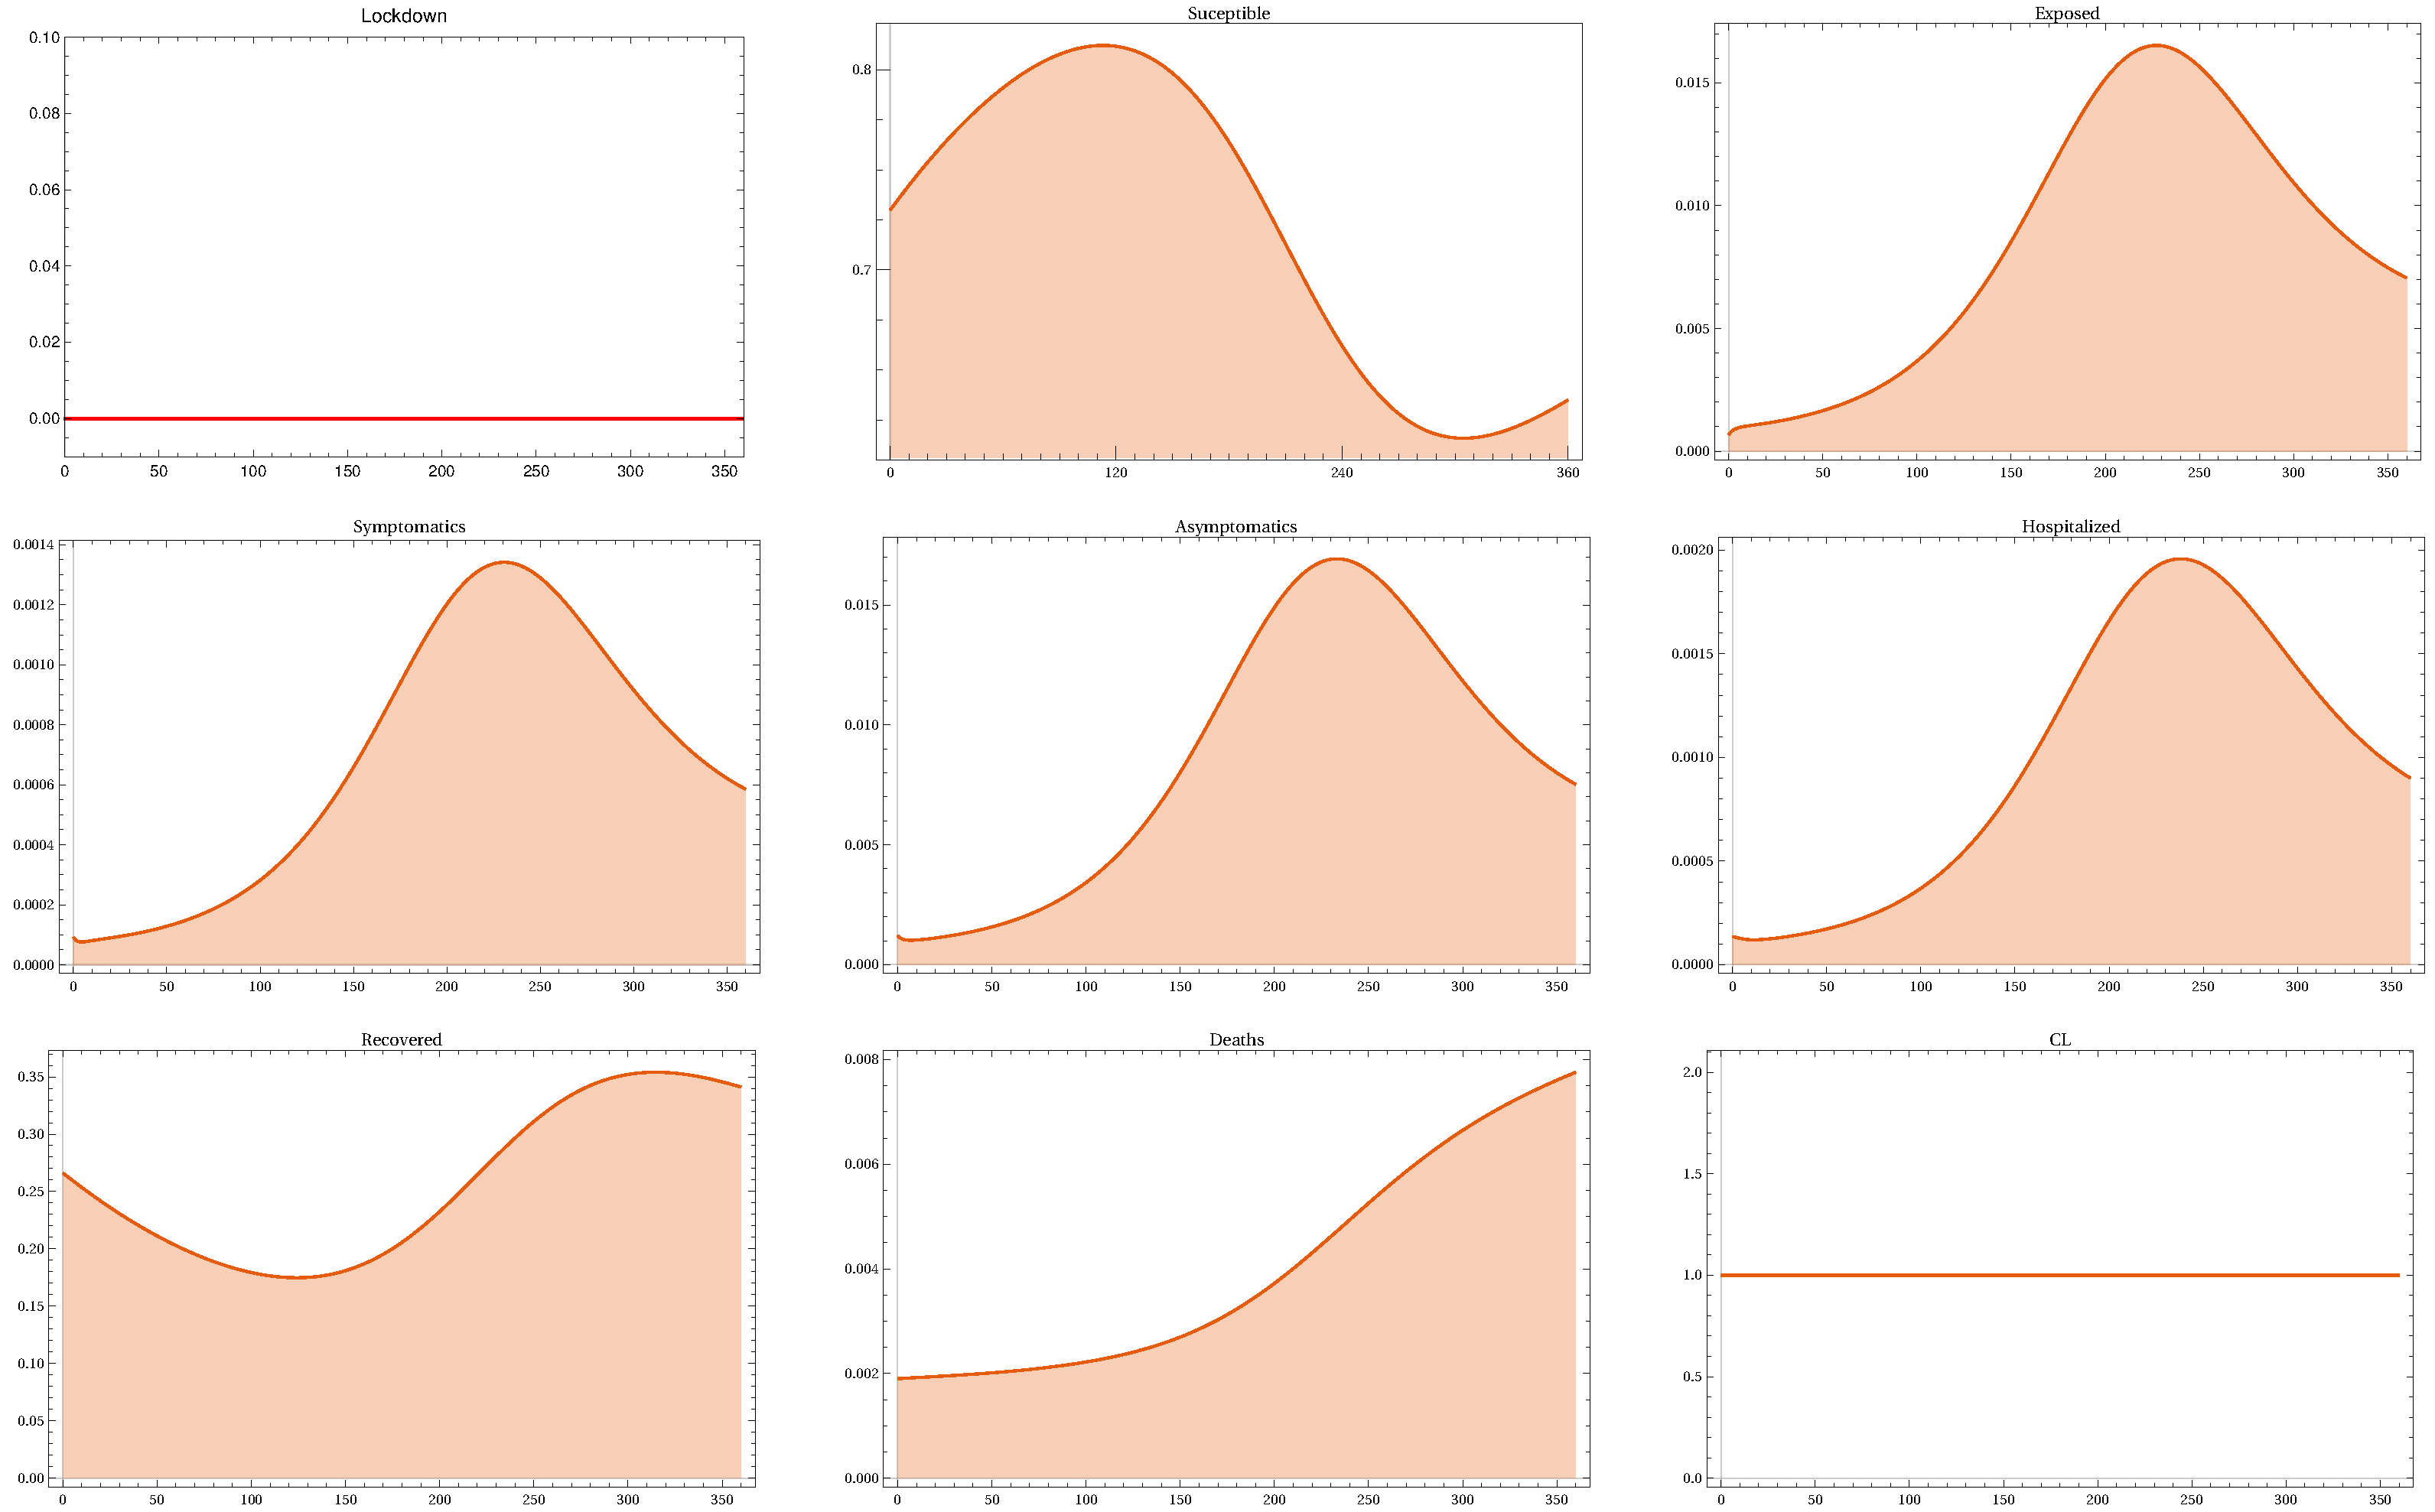
\includegraphics[scale=0.25,
        keepaspectratio]{Figures/no_contraled_dynamics}
    \end{center}
    \caption{
        Spreed dynamics of COVID-19 according to model in
        \Cref{eqn:base_dynamics}.
    }
\end{figure}

     See \Cref{tbl:dynamics_base_parameters} for notation and references
     values.
     \added[id=SDIV, comment={use WPS}]{Put here the flow diagram}
%
\begin{table*}[h!]
	\centering
	\begin{tabular}{>{\centering}%
        p{0.2\textwidth}%
        p{0.4\textwidth}
    }
    \toprule
		\textbf{Parameter} & \textbf{Description}
  	\\
  	\midrule
		$\mu$ &
			Death rate
		\\
        $\beta_S$ &
        	Infection rate between susceptible and symptomatic infected
		\\
        $\beta_A$ &
        	Infection rate between susceptible and asymptomatic infected
		\\
        $\lambda_V$ &
        	Vaccination rate
		\\
        $\delta_{V}^{-1}$ &
        Vaccine-induced immunity
		\\
        $\varepsilon$ &
        	Vaccine efficacy
		\\
        $\kappa^{-1}$ &
        	Average incubation time
        \\
		$p$ &
			New asymptomatic generation proportion
		\\
	    $\theta$ &
        	Proportion of suceptible individuals under lockdown
        \\
        $\gamma_{S}^{-1}$ &
        	Average time of symptomatic recovery
        \\
		$\gamma_{A}^{-1}$ &
			Recovery average time of asymptomatic individuals
		\\
		$\gamma_{H}^{-1}$ &
			Recovery average time by hospitalization
		\\
        $\delta_{R}^{-1}$ &
        	Natural immunity
  		\\
  		$\delta_{H}$ &
        	Infected symptomatic hospitalization rate
  		\\
  	\bottomrule
	\end{tabular}
		\caption{
			Parameters definition of model in
			\Cref{eqn:base_dynamics}.}
    \label{tbl:dynamics_base_parameters}
\end{table*}
%
\begin{figure*}[htb]
    \centering
    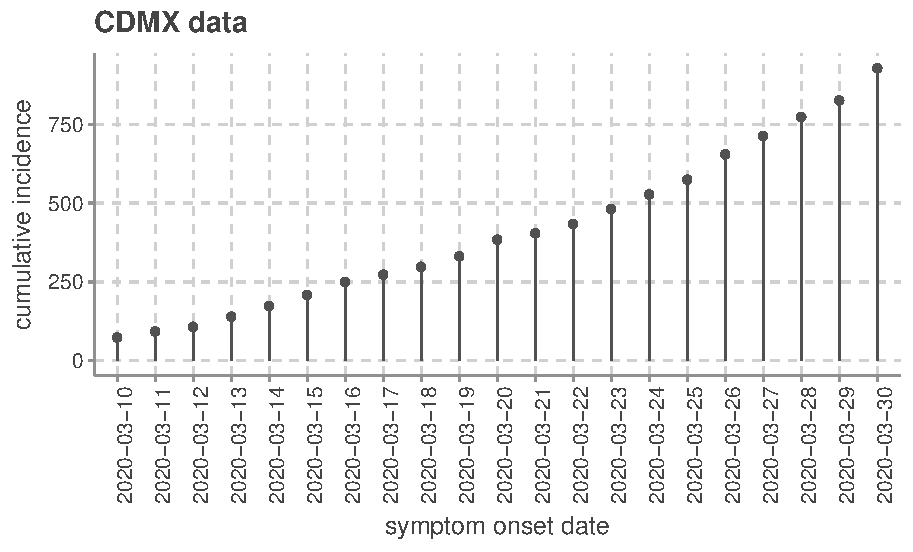
\includegraphics[scale=0.8, keepaspectratio]{Figures/cdmx_input_data}
    \caption{%
        Cumulative new symptomatic and confirmed COVID19 reported cases from
        Ciudad de Mexico and Valle de Mexico
        \cite{cdmxDATA} between March, 10, to March 30 of
        2020.
        \href{https://plotly.com/~AdrianSalcedo/48/}{%
		https://plotly.com/~AdrianSalcedo/48/}
	}
    \label{fig:data_CDMX}
\end{figure*}
%

        \subsection{Parameter calibration}
            %!TEX root = main.tex
\begin{figure*}[htb]
    \centering
    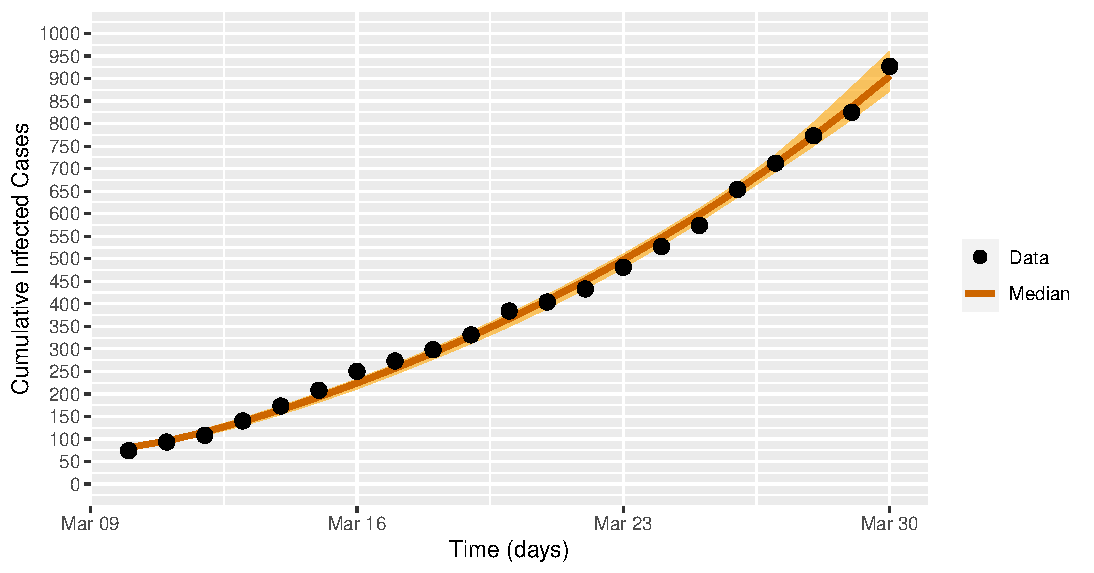
\includegraphics[scale=0.6, keepaspectratio]{./cdmx_CIs_data_begining_fit}
    \caption{%
        Fit of diary new cases of Mexico city
        during exponential growth.
    }
    \label{fig:data_CDMX_fitting}
\end{figure*}
%

\paragraph{Bayesian estimation}
We calibrate parameters of our base dynamics in
\eqref{eqn:base_dynamics} via Multichain Montecarlo (MCMC).
To this end, we assume that the comulative
incidence of new infected symptomatic cases $CI_S$
follows a Poisson distribution with mean $\lambda_t = IC_s(t)$. Further,
following [] we postulate priors for $p$ and $\kappa$
\begin{equation}
    \label{eqn:boservation_model}
    \begin{aligned}
        Y_t & \sim Poisson(\lambda_t),
        \\
        \lambda_t
        &=
        \int_{0}^t p \delta_e E ,
        \\
        & p \sim \text{Uniform} (0.3, 0.8),
        \\
        & \kappa \sim \text{Gamma}(10, 50).
    \end{aligned}
\end{equation}
%
\textbf{}\comment[id=SDIV]{Review this $R_0$ calculation with Gabriel}
Using the reproductive number definition
of Van DenDrishe [CITE], 
and defining $R_1 = \epsilon\theta- \theta +1$, 
$R_2 = \mu + \delta_H+\gamma_S+\mu_{I_{s}}$
we obtain
\begin{equation*}
    \label{eqn:reproductive_number}
    R_0 :=
  \frac{\kappa}{(\kappa+\mu)(\delta_L+\mu)}\left(\mu R_1+\delta_L\right)
  \left[\frac{p\beta_S}{R_2}
  +\frac{(1-p)\beta_A}{\gamma_A+\mu}\right].
\end{equation*}

\Cref{fig:data_CDMX_fitting} displays data of coumulative confirmed cases
of COVID-19 of Mexico city, and \Cref{fig:data_CDMX_fitting} displays the fitt
of our model in \Cref{eqn:base_dynamics,eqn:boservation_model}.
\Cref{tbl:parameters_values} enclose fixed and estimated parameters to this
setting.

  \begin{table*}
    \centering
    \begin{tabular}{@{}llr@{}}
    \toprule
        Parameter
        &   \centering{Median}
        &   Reference
        \\
        \midrule
          $q_r$, $\epsilon$
            &
              \num{.4}, \num{.3}, \num{.1}
            &
              this study
        \\
            $\beta_S$
            & $q_r \times \num{8.690483e-01} $
            & this study
        \\
            $\beta_A$
            & $q_r \times \num{7.738431e-01}$
            & this study

        \\
            $\kappa$
            & \num{0.19607843}
            & $*$
        \\
            $p$
            & \num{0.1213}
            & $*$
        \\
          $\theta$
          & \num{0.2},
          & this study
        \\
          $\delta_L$
          & \num{0.04}
          & postulated
        \\
            $\delta_H$
            &\num{0.2}
            & $*$
        \\
          $\delta_V$
          &\num{ 0.0027397260273972603}
          & $\delta_V ^{-1} = \SI{2}{years}$
        \\
        &&
            CanSinoBIO
        \\
          $\delta_R$
          & \num{0.00555556}
          & $\delta_R^{-1} \approx \SI{180}{days}$
        \\
            $\mu$
            & \num{ 3.913894e-05}
            & $**$
        \\
            $\mu_{I_S}$
            & \num{0.0}
            &
        \\
            $\mu_{H}$
            & \num{0.01632}
            & [FENG]
        \\
            $\gamma_S$
            & \num{0.09250694}
            & $*$
        \\
             $\gamma_A$
             & \num{0.16750419}
             & $*$
        \\
           $\gamma_H$
            & \num{5.079869e-01}
            & $*$
        \\
          $\lambda_V$
          &  \num{0.00061135}
          &
        \\
          $\varepsilon$
          & \num{0.7}, \num{0.80}, \num{0.9}, \num{0.95}
          & [PRESS RELESASES]
        \\
        \midrule
            $N$
             & \num{26446435}
             & $**$
        \\
            $L_0$
            & \num{0.26626009702112796}
        \\
            $S_0$
             & \num{0.463606046009872}
             &
        \\
            $E_0$
             & \num{0.00067033}
             & $*$
        \\
            $I_{S_0}$
            & \num{9.283e-05}
            & $***$
        \\
            $I_{A_0}$
            & \num{0.00120986}
            & $*$
        \\
            $H_0$
            & \num{1.34157969e-04}
            & $**$
        \\
            $R_0$
            & \num{2.66125939e-01}
            &
        \\
            $D_0$
            & \num{0.00190074}
            & $**$
        \\
            $X_{vac}^0$
            & 0.0
        \\
            $V_0$
            & 0.0
        \\
            $Y_{I_S} ^ 0$ &
            \num{0.12258164}
        \\
            $B$
        &
            \num{0.0003592166581242425}
        &
            $
                \displaystyle
                \SI{9500}{beds} / {N}
            $
        \\
          $a_{I_S}$
            & \num{0.0020127755438256486}
            & DALY def
        \\
          $a_{H}$
            & \num{0.001411888738103725},
            or
        \\
        & $
            a_H(x):=
            \num{0.001411888738103725}
            \log(\frac{1}{B - \kappa I_S})
        $
        & DALY def [Jo 2020]
        \\
            $a_D$
            & \num{7.25}
            & DALY def
      \\
        \bottomrule
    \end{tabular}
    \caption{Model parameters. Values based mainly in [FNEG]}
    \label{tbl:parameters_values}
\end{table*}
    \section{Imperfect-preventive COVID-19 vaccination}
        %!TEX root = main.tex
\paragraph{Preventive vaccines}
\paragraph{Efficacy and vaccine-induced immunity}
\paragraph{Actual vaccine stage development}
\paragraph{Vaccination reproductive number}
\paragraph{Vaccination rate $\lambda_V$ estimate}
\paragraph{Feasibility regions according to efficacy and vaccination rate}
%
\begin{equation}
    \label{eqn:vacination_dynamics}
    \begin{aligned}
        L' =&  \theta \mu N^{\star}
                -(\epsilon \lambda + \delta_L + \mu) L 
        \\
        S' =&
        	(1 - \theta) \mu N^\star
            + \delta_L L
            + \delta_V V
            + \delta_R R
        	\\
            &-
            \left(
            	\lambda + \lambda_V + \mu
            \right) S
        \\
        E' =&
                \lambda (\epsilon L + (1-\varepsilon) V + S)
                - (\kappa + \mu) E
        \\
        I_S' =&
        	p \kappa E
            - 
            (	
            	\delta_H +
            	\gamma_S +
                \mu_{I_S} +
                \mu
            ) I_S
        \\
        I_A' = &
                (1 - p) \kappa E - (\gamma_A + \mu) I_A
        \\
        H' = &
        		\delta_H I_S - (\gamma_H + \mu_H + \mu) H
        \\
        R' = &
            	\gamma_S I_S +
                \gamma_A I_A +
                \gamma_H H 
                - (\delta_R + \mu) R
        \\
        D'  = &
                \mu_{I_S} I_S + \mu_H H
        \\
        V' = &
            \lambda_V  S
            - \left[
            	(1 - \varepsilon) \lambda
                + \delta_V
                + \mu
            \right ] V
        \\
        \\
            \frac{dX_{vac}}{dt}
            	&=
            	(u_V(t) + \lambda_V)
            	\left[
            		S + E + I_A + R
            	\right]
        \\
            \frac{d Y_{I_S}}{dt}
            	& = p \kappa E
        \\
            \lambda &:=
                \frac{\beta_A I_A + \beta_S I_S}{N^{\star}}
        \\
        \\
            L(0) &= L_0, 
            \ S(0) = S_0, 
            \ E(0) = E_0, 
        \\
            I_S(0) &= I_{S_{0}},
            I_A(0) = I_{A_{0}},
            H(0) = H_0, 
        \\
            R(0) &= R_0, \ D(0) = D_0,
      \\
            V(0) &= 0, \ X_{vac}(0) = 0, \quad
      \\
            X_{vac}(T) &= x_{coverage},
      \\
            N^{\star}(t) &=
                L + S +E + I_S + I_A +
                H + R + V .
        \end{aligned}
\end{equation}

    \section{Vaccination reproductive number}
        \paragraph{$R_0$ definition}
\paragraph{No  vaccine reproductive number}
\paragraph{Vaccine reproductive number}
\paragraph{Efficacy, coverage and vaccination rate}

\comment[id=SDIV]{%
    Here countor plots figure as function of efficacy and
    vaccination rate%
}
%
\added[id=SDIV]{Here Gabriel's R not calculations.}

\begin{equation*}
 R_{v0} := \left[ 1-\frac{\varepsilon \lambda_V}
 {\mu+\lambda_V+\delta_V}
 -\frac{\theta\mu(1-\epsilon)}{\mu+\delta_L+\lambda_V}\right]
 (\mu R_1+\delta_L)R_0
\end{equation*}
%
\begin{figure*}[tbh]
    \centering
    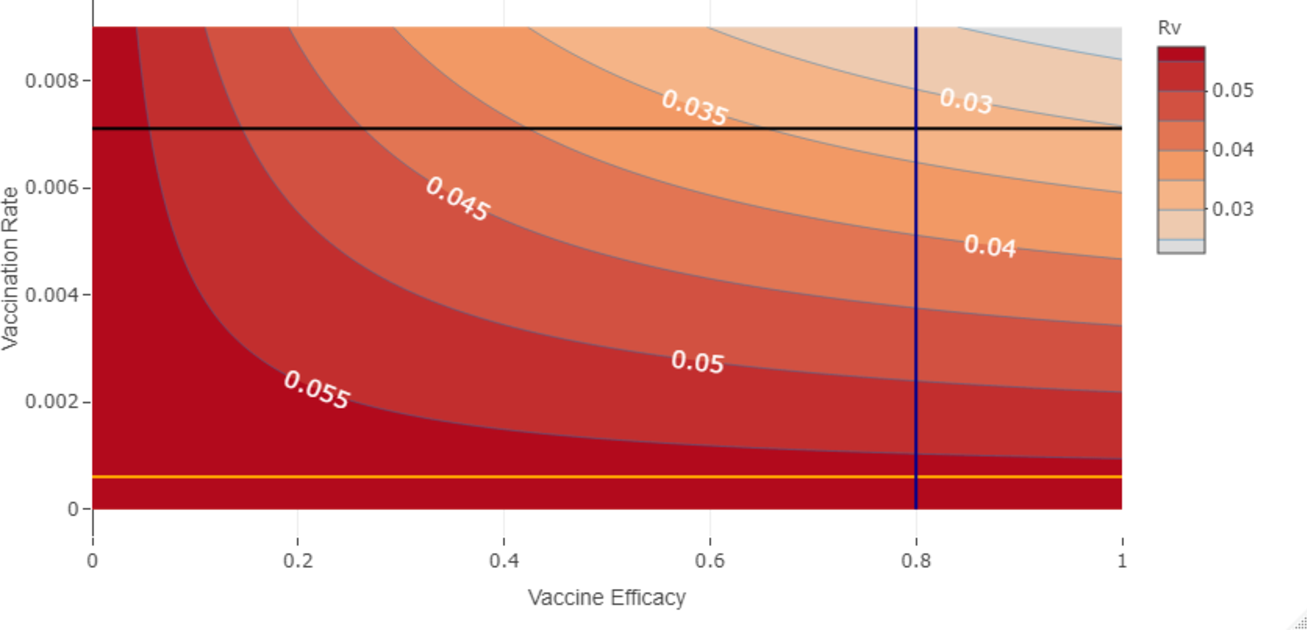
\includegraphics[scale=0.565, keepaspectratio]{Figures/Rv_contour}
    \caption{R not contour plot as function of efficacy and vaccination rate.}
    \label{fig:rvcontour1}
\end{figure*}




    \section{Optimal controlled version}
        %!TEX root = main.tex
\paragraph{Controlled Model}
Now wee model vaccination, treatment and lockdown as a optimal control problem.
According to dynamics in \Cref{eqn:base_dynamics}, we modulate the vaccination
rate with a time-dependent control signal  $u_V(t)$. We add
compartment $X_{vac}$
to count all the vaccine applications of lockdownm susceptible, exposed,
asymptomatic and
recovered individuals. This process is modeled by
\begin{equation}
\label{eqn:counter}
  X'(t) =
    (\lambda_V + u_V(t))(L + S + E + I_A + R)
\end{equation}
and describes the number of applied vaccines at time $t$.
Consider
$$x(t):= (L, S, E, I_S, I_A, H, R, D, V, X_{vac})^{\top}(t)$$
and  control signal $u_v(\cdot)$. We quantify the cost and reward of a vaccine
strategy policy via the penalization functional
\begin{equation}
    \label{eqn:cost_functional}
    J(u_L, u_V):=
        \int _0 ^ T
        a_S p \kappa E(r) +
        a_H \delta_H I_s(r) +
        a_D
        \left[
            \mu_{I_S} I_S(r) + \mu_H H(r)
        \right] +
        \frac{1}{2}
        \left[
            c_L u_L^2(r) +
            c_V u_v^2(r)
        \right]
        dr.
\end{equation}
In other words, we assume in functional $J$ that pandemic cost is proportional
to the symptomatic hospitalized and death reported cases and that a vaccination
and lockdown policies implies quadratic consumption of resources.
\comment[id=SDIV]{Write explication in the context of DALYs}

    Further, since we aim to simulate vaccination policies at different coverage
scenarios, we impose the vaccination counter state's final time condition
$X_{vac}(T)$
\begin{equation}
    \begin{aligned}
      x(T) &= (\cdot, \cdot, \cdot, \cdot, \cdot, X_{vac }(T))^{\top},
      \in \Omega
      \\
      X_{vac}(T)
        &= x_{cover age},
      \\
      x_{coverage}
        & \in
        \left \{
          \text{Low(0.2)},\text{Mid(0.5)}, \text{High(0.8)}
        \right \} .
    \end{aligned}
\end{equation}
    Thus, given the time horizon $T$, we impose that the last fraction of
vaccinated populations corresponds to 20\%, 50\% or 80\%, and
the rest of final states as free. We also impose the path constraint
\begin{equation}
    \label{eqn:path_constrain}
    \Phi(x,t):= H(t) \leq B,
    \qquad \forall t \in [0, T],
\end{equation}
to ensure that healthcare services will not be overloaded. Here $\kappa$
denotes hospitalization rate, and $B$ is the load capacity of a
health system.

    Given a fixed time horizon and vaccine efficiency,
we estimate the constant vaccination rate as the solution of
\begin{equation}
    x_{coverage} = 1 - \exp(-\lambda_V T).
\end{equation}
    That is, $\lambda_V$ denotes the constant rate
to cover  a fraction $x_{coverage}$ in time horizon $T$.
Thus, according to this vaccination rate, we postulate a policy $u_v$ that
modulates vaccination rate according to $\lambda_V$ as a baseline. That is,
optimal vaccination amplifies or attenuates the estimated baseline
$\lambda_V$ in a interval $[\lambda_V ^ {\min}, \lambda_V ^ {\max}]$
to optimize functional $J(\cdot)$\textemdash minimizing
symptomatic, death reported cases and optimizing resources.

    Our objective is minimize the cost functional
\eqref{eqn:cost_functional}\textemdash over an appropriated functional
space\textemdash subject to the dynamics in
\cref{eqn:base_dynamics,eqn:counter}, boundary conditions, and the path
constrain in \eqref{eqn:path_constrain}.
That is, we search for vaccination policies $u_V(\cdot)$, which
solve the following optimal control problem (OCP).
\begin{equation}
    \label{eqn:vital_dynamics}
    \begin{aligned}
        \min_{\mathbf{u} \in \mathcal{U}}
            J(u_L, u_V) := &
                \int_0 ^  T
                    a_S p \kappa E(r) +
                    a_H \delta_H I_s(r) +
                    a_D
                    \left[
                        \mu_{I_S} I_S(r) + \mu_H H(r)
                    \right]
                dr +
        \\
                &
                \int_0^T
                    \frac{1}{2}
                    \left[
                        c_L u_L^2(r) +
                        c_V u_v^2(r)
                    \right]
                    dr.
        \\
            \text{s. t.} &
        \\
            L' & =  \theta \mu N^{\star}
                -\epsilon \lambda L - u_L(t) L - \mu L
        \\
            S' & =
                (1 - \theta) \mu N^\star
                + u_L(t) L
                + \delta_v V
                + \delta_R R
        \\
                & \qquad -
                \left[
                \lambda + (\lambda_V + u_V(t)) + \mu
                \right] S
        \\
            E' &=
                \lambda (\epsilon L + (1-\varepsilon) V + S)
                - (\kappa + \mu) E
        \\
            I_S' &=
                p \kappa E
                % + (1 - q) \gamma_M M(t)
                - (\gamma_S +
                    \mu_{I_S} +
                    \delta_H +
                    %u_M(t) +
                    \mu) I_S
        \\
            I_A' &=
                (1 - p) \kappa E - (\gamma_A + \mu) I_A
        \\
            H' &=
                \delta_H I_S - (\gamma_H + \mu_H + \mu) H
        \\
            R'  &=
                \gamma_S I_S +
                \gamma_A I_A +
                \gamma_H H % +
                - (\delta_R + \mu) R
        \\
            D' &=
                \mu_{I_S} I_S + \mu_H H
        \\
            V' &=
                (\lambda_V + u_V(t)) S
                - \left[
                (1 - \varepsilon) \lambda
                + \delta_V
                + \mu
                \right ] V
        \\
        \\
            \frac{dX_{vac}}{dt}
                &=
                (u_V(t) + \lambda_V)
                \left[
                    L + S + E + I_A + R
                \right]
        \\
            \frac{d Y_{I_S}}{dt}
                & = p \kappa E
        \\
            \lambda &:=
                \frac{\beta_A I_A + \beta_S I_S}{N^{\star}}
        \\
        \\
            L(0) &= L_0,
            \ S(0) = S_0,
            \ E(0) = E_0,
            \ I_S(0) = I_{S_{0}},
      \\
            I_A(0) &= I_{A_{0}},
            H(0) = H_0, \
            \ R(0) = R_0, \ D(0) = D_0,
      \\
            V(0) &= 0, \ X_{vac}(0) = 0, \quad
            u_V(.) \in [u_{\min}, u^{\max}],
      \\
            X_{vac}(T) &= x_{coverage},
      \quad
            \kappa I_S(t) \leq B, \qquad
            \forall t \in [0, T],
      \\
            N^{\star}(t) &=
                L + S +E + I_S + I_A +
                H + R + V
        \end{aligned}
\end{equation}

The policies we are considering in the OCP are piecewise constant; see the Appendix for details. OCPs with this class of policies have been
    studied in different contexts. For instance, a solution method based on the
    gradient of the cost functional is studied in \cite{MR3223602}; convergence
    results of piecewise constant solutions to permanent solutions in
    linear-quadratic problems are given in \cite{MR3627992}; or, in
    \cite{CANTUNetAl}, a general numerical methodology to find piecewise
    constant solutions is proposed. In fact, to find the optimal policies we use the methodology \cite{CANTUNetAl}. Even though the existence of solutions to OCPs in the class of piecewise constant policies is known, for completeness, we sketch a straightforward proof in the Appendix under assumptions that hold for the OCP described above.   



    \section{Numerical Experiments}
        
\comment[id=SDIV]{Aqui va tu descripcion Frank. }
        \begin{figure*}
    \centering
    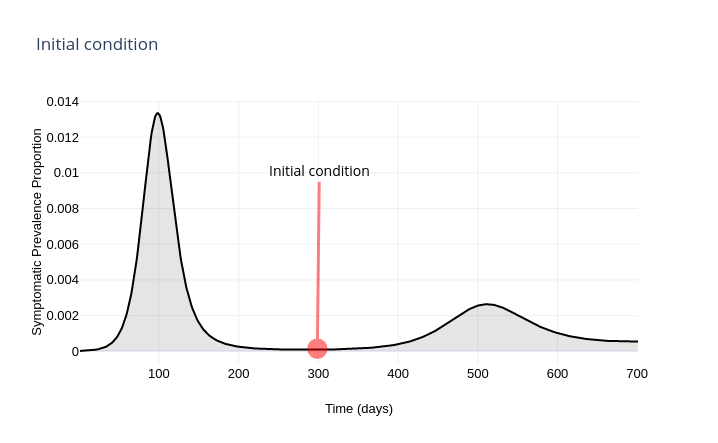
\includegraphics[scale=0.5, keepaspectratio]{figs/InitialCondition}
    \caption[Initial condition]{
        Initial condition scheme. We assume a positive
        prevelance. Forreference, at the date of write this manuscript,
        prevalence in CDMX is
        around \SI{16000}{cases}, see
        \href{https://plotly.com/~sauld/36/}{https://plotly.com/~sauld/36/}
        to display a electronic viewer.}
        \label{fig:initialcondition}
\end{figure*}

\begin{figure*}[tbh]
    \centering
    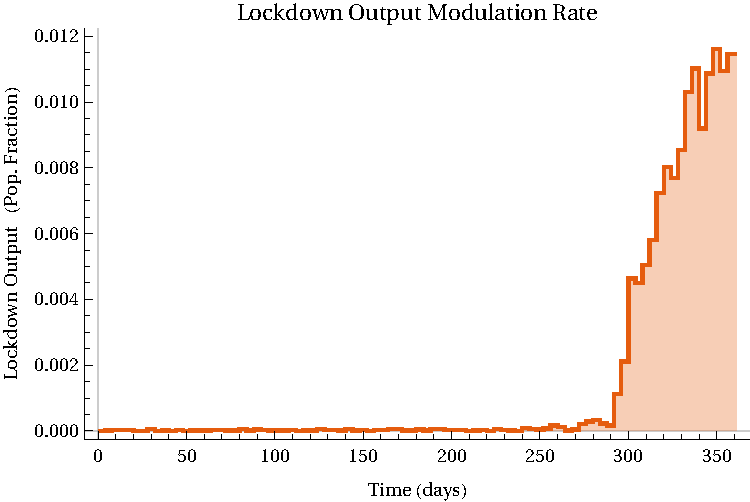
\includegraphics[width=0.7\linewidth]{figs/lockdown_control_signal}
    \caption[Lockdown modulation signal.]{Lockdown modulation signal.}
    \label{fig:lockdowncontrolsignal}
\end{figure*}

\begin{figure}
    \centering
    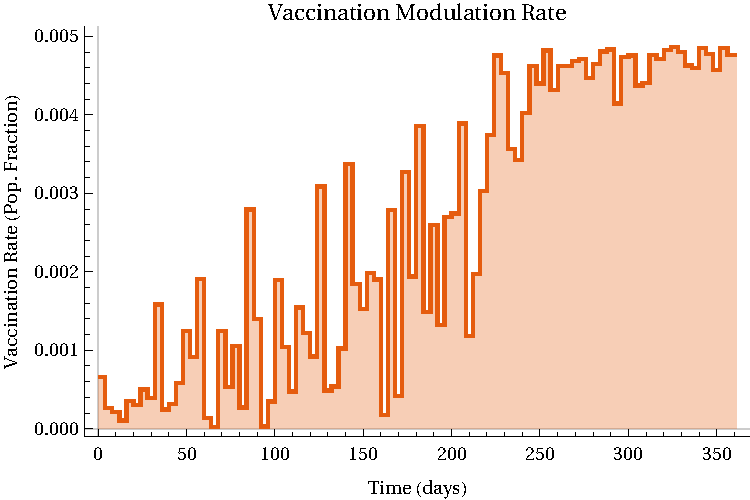
\includegraphics[width=0.7\linewidth]{figs/Vaccination_control_signal}
    \caption[Vaccination rate modulation.]{Vaccination rate modulation.}
    \label{fig:vaccinationcontrolsignal}
\end{figure}

\begin{figure}[tbh]
    \centering
    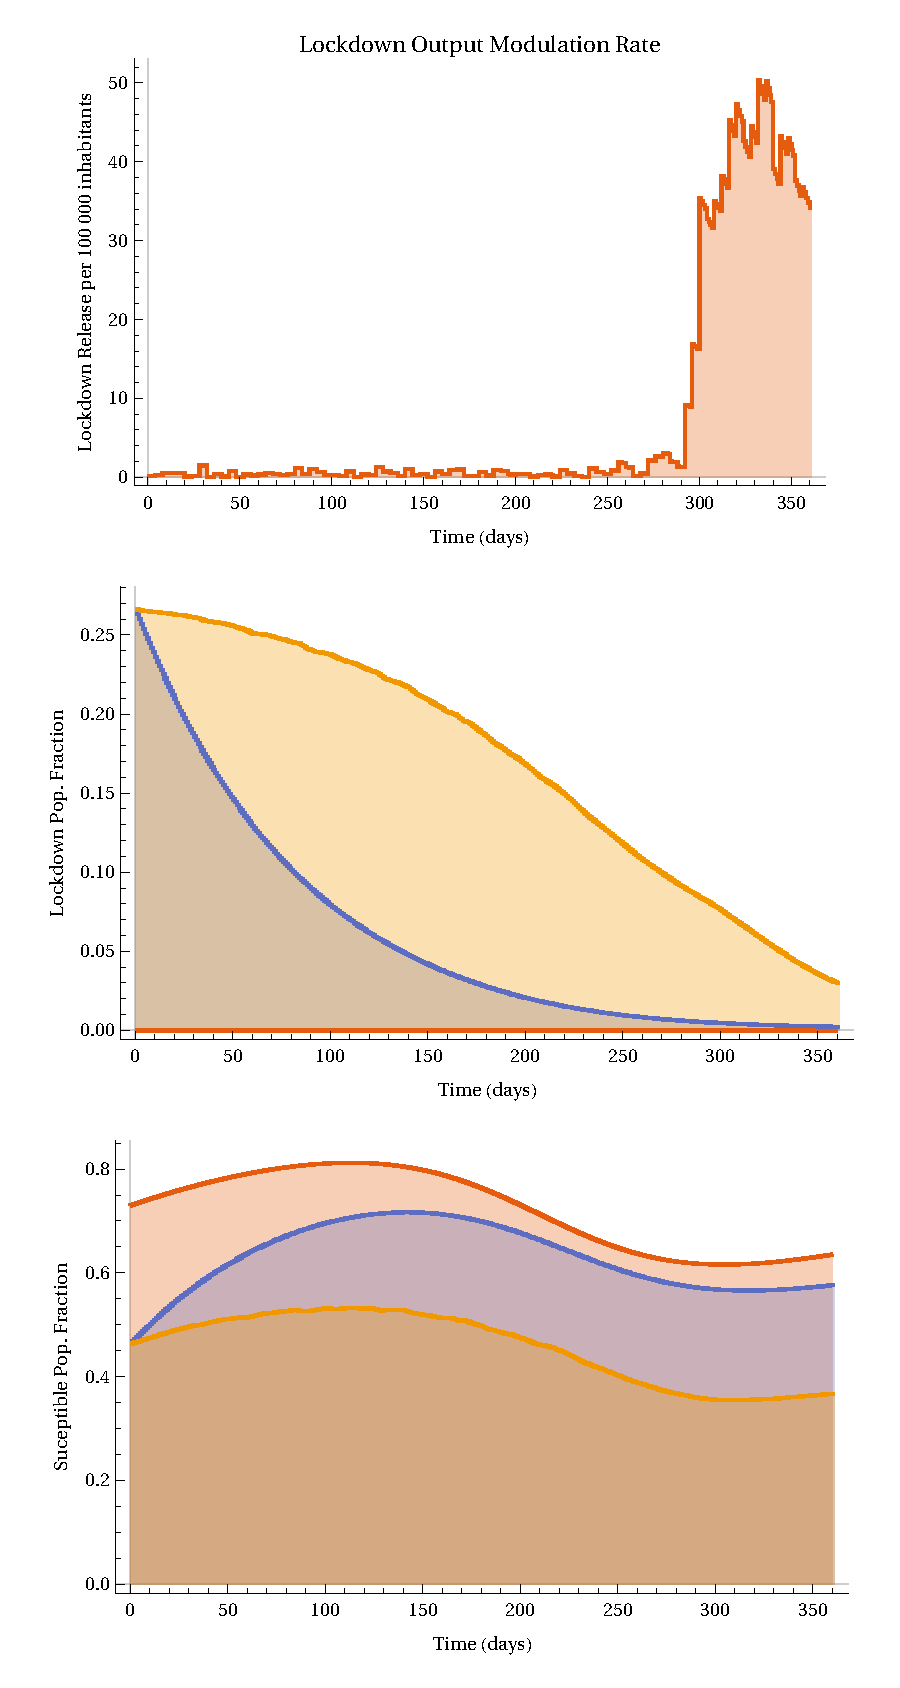
\includegraphics[width=1.0\linewidth]{figs/LockdownEffect}
    \caption{Modulation lock down release.}
    \label{fig:lockdowneffect}
\end{figure}

\begin{figure*}[tbh]
    \centering
    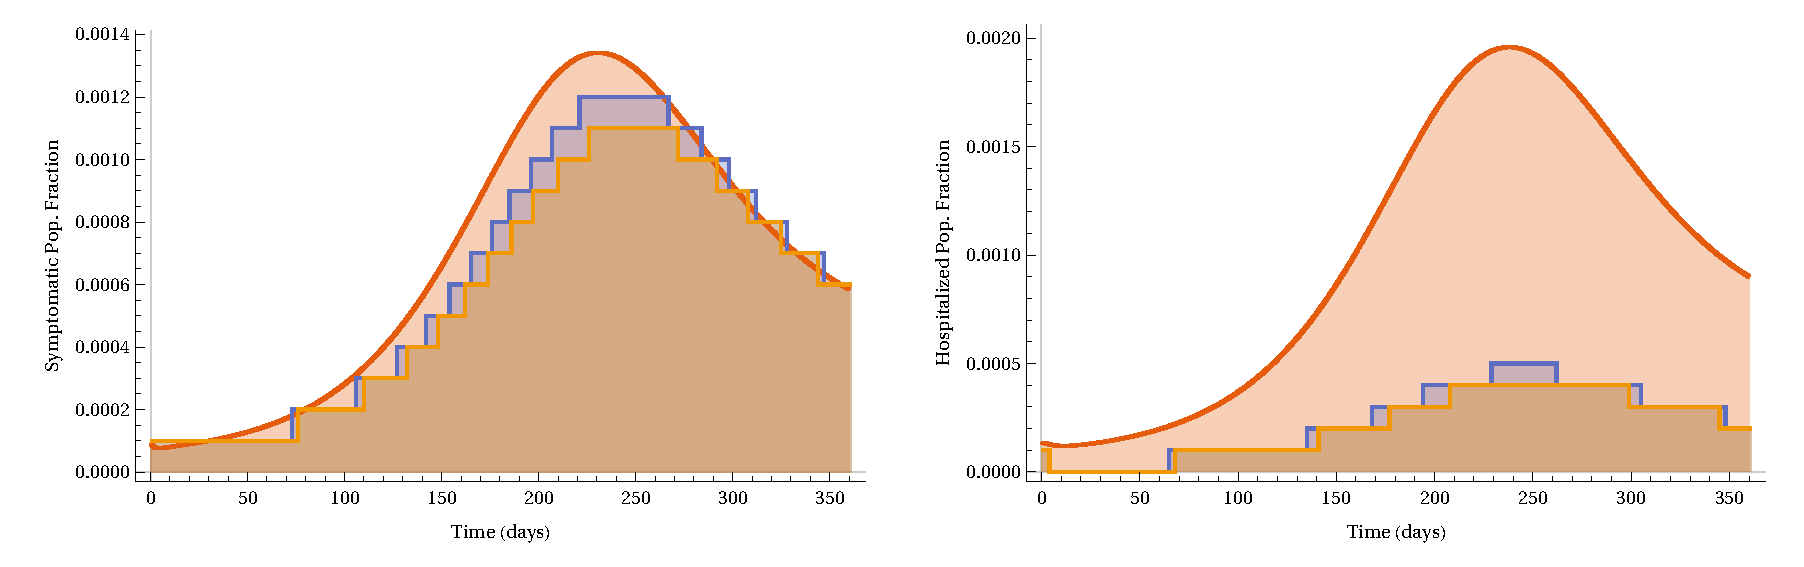
\includegraphics[width=1.0\linewidth]{figs/VaccinationEffect}
    \caption{Symptomatic Prevalence and Hozpitalization.}
    \label{fig:vaccinationeffect}
\end{figure*}


    \listofchanges[style=compactsummary]
    \appendix
  \section{Existence of optimal policies}
    %!TEX root = main.tex
In this appendix, we show the existence of optimal policies in the class of
{\it piecewise constant policies}. Consider the following cost functional that
we want to minimize
\begin{equation}\label{costFunctional}
  \int_0^T C(X(t),u(t)) dt
\end{equation}
subject to the dynamics
\begin{equation}\label{dynamics}
  \dot{X}(t) = f(X(t),u(t)),  \qquad    0\leq t \leq T,
\end{equation}
and the initial state $X(0)=x_0$. The functions $u:[0,T]\to U$ are called {\it
control polices}, where $U$ is a subset of some Euclidean space.
    %The
    %cost functional \eqref{eqn:cost_functional} and the dynamics
    %\eqref{eqn:vital_dynamics} are particular cases of \eqref{costFunctional}
    %and \eqref{dynamics}, respectively.
%
Let $t_0<t_1<\ldots <t_n$, with
$t_0=0$ and $t_n=T$, be a partition of the interval $[0,T]$.
We consider piecewise constant policies $\tilde{u}$ of the form
\begin{equation}\label{PieceConstCont}
  \tilde{u}(t) = a_j\qquad t_j\leq t < t_{j+1}
\end{equation}
 for $j=0,\ldots,n-1$.
\begin{assumptions}
    We made the following assumptions.
    \begin{enumerate}[({A}-1)]
        \item
            The function $f$ in the dynamics \eqref{dynamics} is of
            class $C^1$.
        \item
            The cost function $C$ in \eqref{costFunctional} is continuous and
            the set $U$ is compact.
    \end{enumerate}
\end{assumptions}
%

    By Assumption (A-1)\textbf{}, the system
\[
  \dot{X}(t) = f(X(t),a_0), \quad X(0)=x_0, \qquad    0\leq t \leq t_1,
\]
has a unique solution $\tilde{X}_0(t;x_0,a_0)$ which is continuous in
$(x_0,a_0)$; see, for instance \cite{Kong2014}.  Next, put $x_1:=\tilde{X}_0(t_1;x_0,a_0)$ and consider the system
\[
  \dot{X}(t) = f(X(t),a_1), \quad X(t_1)=x_1, \qquad    t_1\leq t \leq t_2,
\]
Again, by Assumption (A-1), the latter system has a unique solution
$\tilde{X}_1(t;x_1,a_1)$ which is
continuous in $(x_1,a_1)$. By following this procedure, we end up having a
recursive solution
\begin{equation*}
  \begin{aligned}
    & \tilde{X}_{n-1}(t;x_{n-1},a_{n-1}),
    \qquad t_{n-1}\leq t \leq T,\\
    & x_{n-1}:=\tilde{X}_{n-2}(t_{n-1};x_{n-2},a_{n-1}),
  \end{aligned}
\end{equation*}
where $\tilde{X}_{n-1}$ is continuous in $(x_{n-1},a_{n-1})$.


For a control $\tilde{u}$ of the form \eqref{PieceConstCont} and the
corresponding solution path $\tilde{X}$, we have
\[
  \int_0^T
    C(\tilde{X}(t),
    \tilde{u}(t)) dt =
      \sum_{j=0}^{n-1}
        \int_{t_j}^{t_{j+1}}
        C(\tilde{X}_j(t),a_j) dt.
\]
Notice that each $\tilde{X}_j$ is a continuous function of $(a_0,\ldots,a_j)$
and $x_0$.

By Assumption (A-2), the mapping
\[
  (a_0,\ldots,a_{n-1})
  \mapsto
  \sum_{j=0}^{n-1}
  \int_{t_j}^{t_{j+1}} C(\tilde{X}_j(t),a_j) dt
\]
is continuous. Since each piecewise constant policy $\tilde{u}$ of the form
\eqref{PieceConstCont} can be identified with the vector $(a_0,\ldots,a_{n-1})$
in the compact set $U\times\cdots\times U$, the functional
\eqref{costFunctional} attains its minimum in the class of piecewise constant
policies.

    The cost functional \eqref{eqn:cost_functional} and the dynamics
\eqref{eqn:base_dynamics} are particular cases of \eqref{costFunctional} and
\eqref{dynamics}, respectively, and satisfy Assumptions (A-1) and (A-2). Then
there exists an optimal vaccination policy of the form \eqref{PieceConstCont}.
  \bibliography{NovelCovid19.bib}
  %\bibliographystyle{plain}
  \bibliographystyle{elsarticle-num}
  
\end{document}
